
\documentclass[a4paper,twocolumn,conference]{IEEEtran}


% *** GRAPHICS RELATED PACKAGES ***
%
\ifCLASSINFOpdf
   \usepackage[pdftex]{graphicx}
  % declare the path(s) where your graphic files are
   \graphicspath{{fig/}}
  % and their extensions so you won't have to specify these with
  % every instance of \includegraphics
  % \DeclareGraphicsExtensions{.pdf,.jpeg,.png}
\else
  % or other class option (dvipsone, dvipdf, if not using dvips). graphicx
  % will default to the driver specified in the system graphics.cfg if no
  % driver is specified.
  % \usepackage[dvips]{graphicx}
  % declare the path(s) where your graphic files are
  % \graphicspath{{../eps/}}
  % and their extensions so you won't have to specify these with
  % every instance of \includegraphics
  % \DeclareGraphicsExtensions{.eps}
\fi

\usepackage{multicol}
\usepackage{url}
\usepackage{graphicx}

\hyphenation{op-tical net-works semi-conduc-tor}

\begin{document}

% paper title

\title{Best of Two Worlds: Reinforcing NaaS Capability with Software-defined Networking}


\author{\IEEEauthorblockN{Feng Liu}
	\IEEEauthorblockA{%Munich Network Management Team\\
		Leibniz Supercomputing Centre (LRZ)\\
		Garching b. M\"unchen, Germany}

%\and

%\IEEEauthorblockN{Hao Yu}
%\IEEEauthorblockA{Department of Photonic Engineering\\
%Technical University of Denmark Denmark\\
%2800 Kongens Lyngby, Denmark}
}

\maketitle


\begin{abstract}
	In this paper we argue that adding SDN-capability to NaaS can significantly enhance
its management flexibilities and offer new service opportunities both for
administrators and users of on-demand network services enabled by NaaS. We
describe our approach to integrate Network-as-a-Service (NaaS) with
Software-defined networking (SDN). Specific envisioned
enhancements through SDN are explained in details and an integration
methodology and architecture are presented.

%
%Our discussion is based on the OpenNaaS
%platform implemented by EU FP7 Mantychore project~\cite{mantychore}.
%

\end{abstract}

\IEEEpeerreviewmaketitle

\section{Introduction}
	\label{introduction}

Flexible network infrastructures are crucial part for today's IT landscape.
Advance in hardware technologies constantly improves performance of
networking devices to suite the needs of applications and accommodate
simultaneous traffic flows. On the other hand, usage scenarios of today's
network infrastructures are very dynamic,ranging from networking for cloud
computing and Network Functions Virtualization (NFV) to deal with short-lived
network traffic spikes such as flash-crowd effect, providers should react agilely to
frequently changing user requirement on networks. This requires more flexibilities
in configuration as well as provisioning of resources in a very short time due
to limited reaction time. 

Considering those two aspects, an ultimate challenge currently faced by network
service providers today is thus how to deliver dynamic network infrastructures
at relatively low costs and in a timely manner. Furthermore network element should be 
application-aware as well, which means requirements from high level applications should 
be considered and reflected in the underlying network infrastructure.
%Such flexible and on-demand
%infrastructures are also required to address individual needs depend on usage
%scenario set by users and their specific applications. 
Obviously traditional network paradigm which purely based on dedicated
networking hardware is not efficient to address this challenge due to
its lacking of flexibility and reconfigurability. Recently a paradigm called
Network-as-a-Service (NaaS)~\cite{naas} which based on network virtualization
technology, shreds lights on this problem. With a layer of software entity,
NaaS paradigm allows creation of virtualized switches, routers and optical
devices ect. using physical devices, thus enables multiple tenants to use a
slice of shared resources according to their specific needs. NaaS can be
seamlessly integrated into other virtual services such as cloud computing and
NFV. NaaS allows more control of network elements from users' perspective of
view. Despite its conceptual advantages, it is still an unsolved question that
how to efficiently control physical network resources in a fine-granulate and precise 
way. 
%
%In order to allow National Research and Education Networks (NREN) and other 
%e-Infrastructure providers across Europe to collaborate and support research communities
%with highly flexible network infrastructures, a framework based on the paradigm of 
%NaaS is created by FP7 Mantychore project. The framework is called OpenNaaS~\cite{opennaas}.
%

A recent effort towards programmable networks with Software-defined networking
(SDN) has attract vast research interests. The idea of separation of data
forwarding and control plane of networking devices can improve controllability
and manageability of networks drastically. If properly integrated, we believe
such flexibility can extent the management and usage of NaaS thus provides as a
plausible solution for sustain the network controls of physical network
devices.  In this paper, we analyze the advantages of integration of SDN into
NaaS paradigm and how such integration can be properly designed and
implemented. The main contribution of this work are:

\begin{itemize}
	\item Proposing an architecture which integrates SDN into NaaS;
	\item Sustaining and enhancing functionalities of NaaS with refined network controls;
	\item Convergence of network infrastructures with cloud computing and NFV.
\end{itemize}

This paper is organised as followings: Section \ref{background}
provides briefly background information regarding NaaS and its use cases;
in Section \ref{naas-sdn} we discuss in-depth on enhancements of OpenNaaS with
support of SDN technology and in the meanwhile provides detailed design of
integration; Section \ref{architecture} and  Section \ref{impl} both detailed
discussion on architecture and a prototypical simulation result is presented;
this paper is concluded by discussion on future works. 


\section{Background: NaaS}
	\label{background}

	\subsection{NaaS}
		
%\begin{figure}[htp]
%	\centering
%	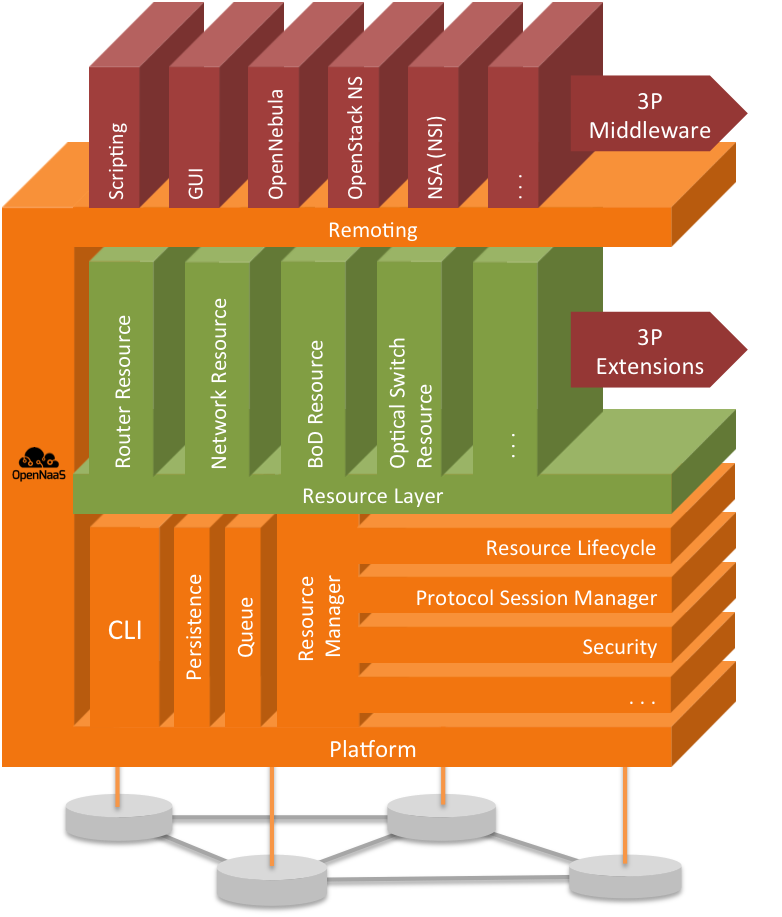
\includegraphics[scale=0.4]{architecture.png}
%	\caption{OpenNaaS Architecture}
%	\label{fig:opennaasarchi}
%\end{figure}


	\subsection{Use Cases}
		\input{use-cases}
	
	



\section{Enhancing NaaS Service with SDN}
	\label{naas-sdn}

Having the concpet and architecture of OpenNaaS presented, in this section we
focuse on enhancements that highlight OpenNaaS serivce withSDN technology and
corresponding functional requirements are derived from those enhancements. 

\subsection{Enhancements}
	
	\subsubsection{Programmable Virtual/Physical Network Appliances}

	The separation of control and data-forwarding mechanisms allows more flexible control
	of packet-forwarding devices. Comparing to classical way of managing
	network devices, behaviour of SDN-compatible devices can be programmed
	through their north-bound interfaces on centralised management station. A
	SDN switch, for example, can be easily programmed to behaviour not only
	packet forwarding device, but also as a firewall or a load-balancer. The
	instructions can be realized in just few lines of code. 

	For OpenNaaS framework, a set of SDN-compatible devices can be programmed
	into different network appliances \emph{according to usage scenarios}.  In
	this way, programmable network can not only be reused but also aggregated
	or split in an on-the-fly manner which provide flexibility from both user
	and administrator perspective of views. Additionally middle-boxes could be
	replaced by unified, programmable and multi-purposed devices, which
	simplifies management and maintenance as well. 

	
	\subsubsection{Refined NaaS Control of Network Resources}

	Management rules and policies can be explicitly stated and enforced using
	proper programming or configuration languages, e.g. \cite{maple, frenetic}.
	Rules can be inserted into device's flow table where forwarding mechanism
	behaves accordingly, for example if data packets with certain origins have
	to traverse through a pre-determined switches can be expressed as flow
	rules.

	In terms of OpenNaaS, a refined control of network resources can
	dramatically reduce the overhead for administrator to configure networks
	with complex user requirement. Policies can be singly used or even be
	negotiated with user to adapt to their needs.

	\subsubsection{Incorporating Advanced Analytics of Networks Behaviors}

	SDN technology inherently facilitates in-network information gathering and
	analysis in order to gain deeper insights of network behaviours and event
	in real-time. Current OpenFlow specification~\cite{of14} for example,
	allows asynchronous and symmetric messages to be sends from devices to
	controller which contain network events such as \texttt{Packet-in/out},
	\texttt{Port-status}, \texttt{Flow-Removed} etc. Given availability of such
	types of messages provided by the resource layer devices, complex analytics
	can be done in order to assist either human operators or automated
	mechanisms to understand network behaviours and reacts to network event if necessary. 
	Analytics can be done either at controller layers at integral part of network OS 
	or controller can simply make those data available through its northbound interface 
	for the above layer to conduct analysis. Note that depending on the scenario, deluge of 
	data may be required to be processed in a real-time in order to achieve the goal, thus
	analytics in network is also an across research area with big data.

	
	\subsubsection{Incorporating QoS into on-demand Network}

	With support of configuration or programming languages, QoS requirements of
	network services created by NaaS can be expressed explicitly as rules in
	flow tables so that QoS policies are reflected and realized, for example
	the control of bandwidth for NaaS virtual networks with different quality
	and load-balancing requirements could be enforced using SDN rules expressed
	in the form of functions \cite{pyretic} as in conventional programming
	languages. 
	

	\subsubsection{Enabling Multi-domain SDN/OpenNaaS Service}
	
	Networking capabilities represented by both virtual and physical devices or
	resource slices can be orchestrated to form complex networking services.
	Since state-of-the-art SDN specification does not support inter-domain
	networking, using other inter-domain capable resources allows SDN networks
	in a single domain to forward their data packet to other domains, for
	instance, if particular kind of traffic must be routed outside of its own
	domain, an underlying SDN switches can be programmed with inter-domain
	routing capabilities such as EGP or BGP, for example a SDN-based inter-domain
	data exchange component at the edges of an organization can be a potential solution
	to allow multi-domain NaaS service. 
	
	\subsubsection{Allowing Continuum in the Network Management}

	Continuum in the network management refers to implementation and refinement
	of management policies or rules from high-level perspective to low-level
	executable management actions. Due to lack of an unified method, providing
	a consistent network management continuum is currently difficult, if at all
	possible. For services such as NaaS, a flexible control has to be in place
	in order to allow administrators to re-configure the network resources to
	adapt to ever changing management policies. A set of executable actions
	down to network interfaces level must be resulted to reflect the change of
	policy changes. With SDN policy languages such as Pyretic~\cite{pyretic}, a
	solid foundation could be built to express network management intentions
	in terms of a unified programming scripts in a generic way, programming
	language concepts such as functions and classes can be used to express the
	management rules and policies.


	\subsubsection{Intelligent Network Management with SDN}

	As underlying technology for NaaS platform, SDN works as a flexible
	intermediate layer between high-level services offered by NaaS and
	low-level infrastructures, e.g. switching/routing hardwares.  In a highly
	utilized NaaS environment, SDN devices may generate a large number of
	events and messages from OpenFlow channels, for example, asynchronous and
	symmetric messages sent back and forth between controller and data layers.
	Those message carries important management information that reflects the
	current behavior, such as changes, faults such as mis-configurations and
	even security informations. Thus aggregation, correlation and in-depth
	comprehension of such messages is of vital importance for understanding the
	performance of network in a real-time manner. It is also a great assistant
	for activities such as debugging of network failures or finding bottle neck
	of networks.  Obviously this is not a trivial task, sheer mount of data and
	complex inter-correlation of data require the processing algorithms to be
	capable of dealing with such data deluge in a highly efficient manner.
	Methods available to data-mining and machine learning researches can be
	explored for this purpose.
	
\subsection{Requirements}


\section{Solution Architecture}
	\label{architecture}
In this section, we present the architecture of adapting SDN-capability to
OpenNaas framework,in which we try to answer following technical questions:

\begin{figure*}[ht]
	\centering
		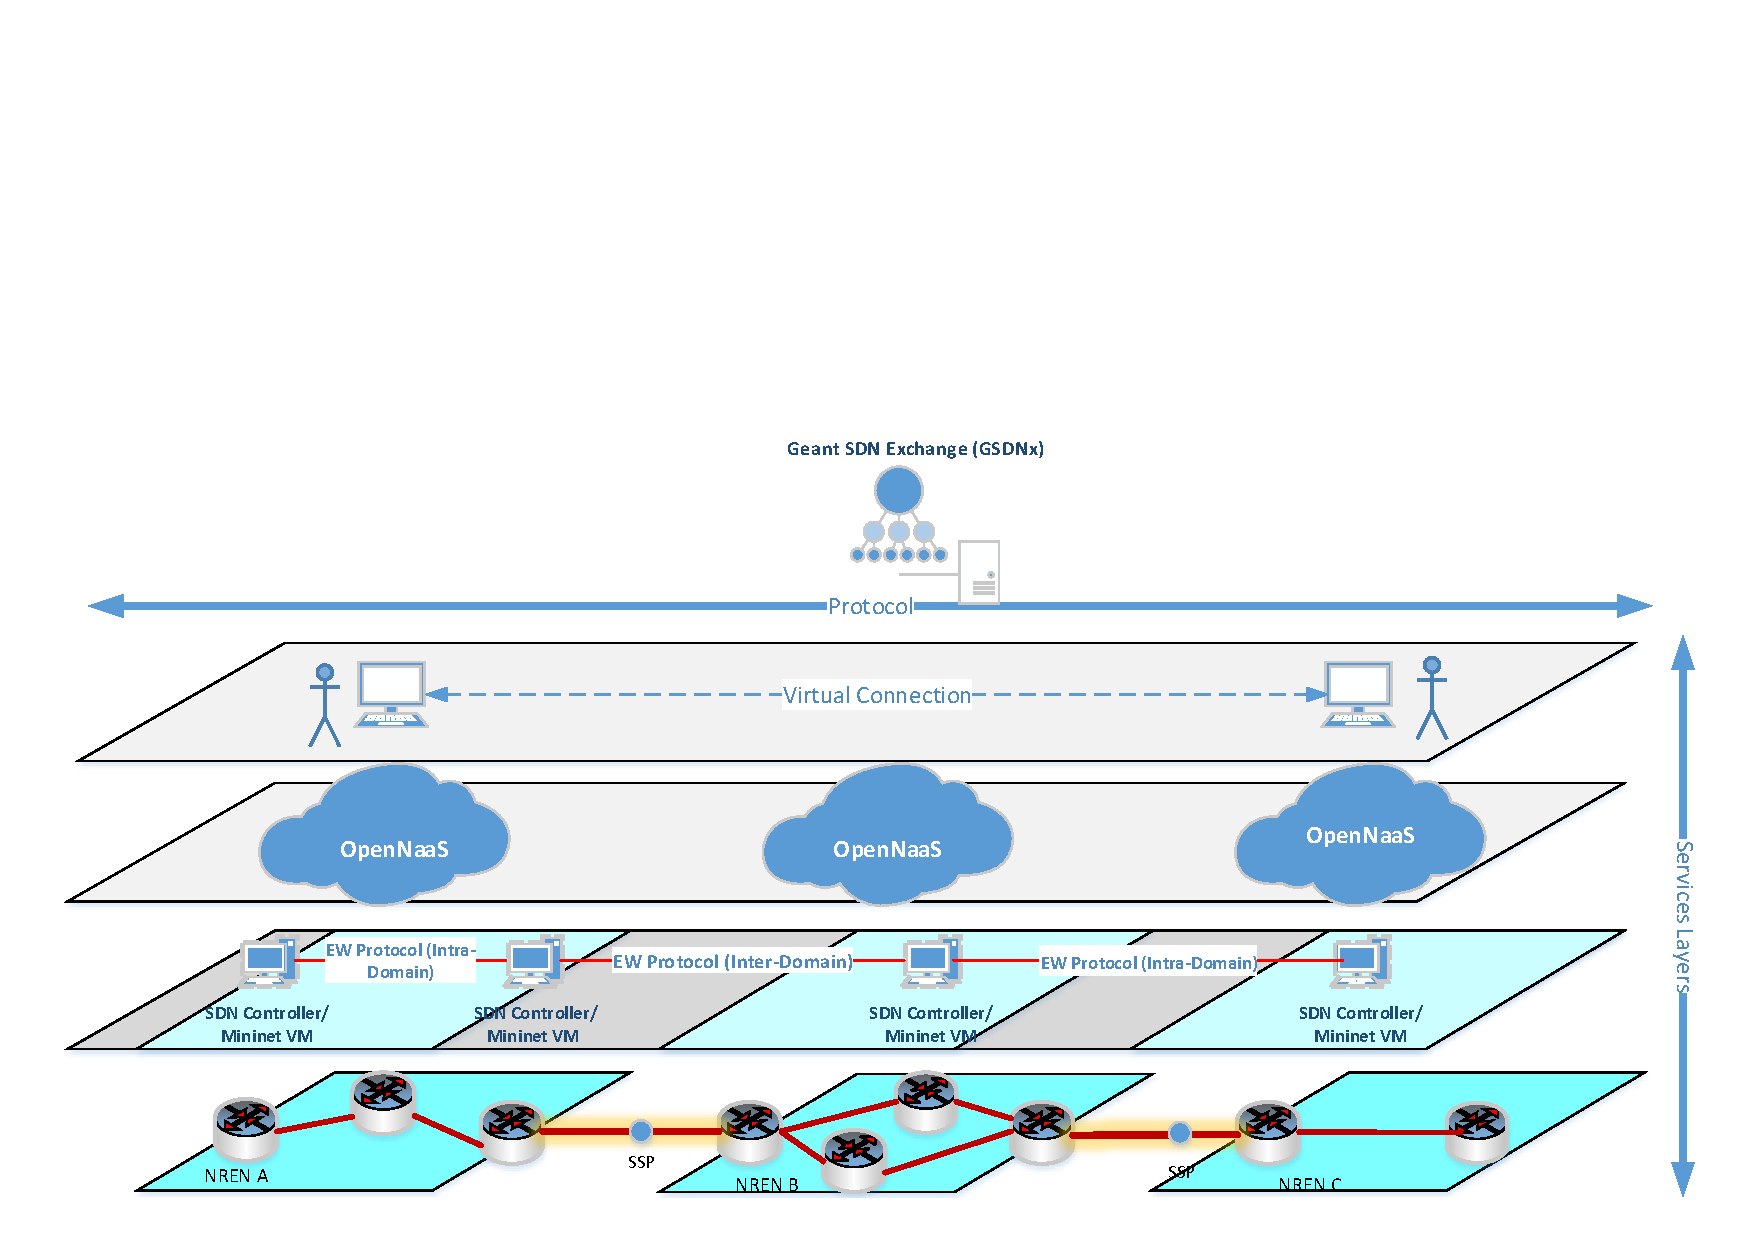
\includegraphics[width=0.7\textwidth]{GN_SDN_NaaS_Architecture.pdf}
	\caption{Architecture of Inter-domain NaaS Service over SDN Facilities}
	\label{fig:arch}
\end{figure*}

\begin{itemize}
	
	\item How to model and architect SDN-based OpenNaaS framework? 
	\item How to properly map SDN components to OpenNaaS framework?
	\item How could SDN-compatible networking devices expose their control primitives to
OpenNaaS framework and in what granularity?
	\item How to represent SDN abstractions to users and administrators of OpenNaaS framework? 

\end{itemize}

\subsection{An Architecture for Building NaaS over SDN Facility}

Figure~\ref{fig:arch} illustrates our proposal of integrating NaaS service over
SDN facilities over multiple domains. We structure the proposed architecture
into functional/service layers, where each layer provides services to its above
layers. Within layers, protocols are used to facilitate information exchanges
between different participants. Explanation regarding each layer is given as
following:

\subsubsection{Resource Layer} At bottom level of the proposed architecture,
basic data packets forwarding  capability allows simple data forwarding either
within or between domains. Note that at this layer, no routing decision is made
regarding the destinations of packets, it simply forwards data packets
according rules that are determined by the controller, thus we say the resource
layer provides data-forwarding serviced by implements rules made by the control
layer, e.g. using OpenFlow protocols. 

\subsubsection{Control Layer} The behavior of data forwarding devices at
resource layer is defined by the control layer, where standard protocol can be
used to define and communicate forwarding rules to devices forwarding table.
It is important to notice that current specifications and standards of OpenFlow
for example, do not consider East-West(EW) communications, thus collaboration
between controller is difficult, if not impossible. We argue that integration
of controller-to-controller protocols will be vital sheer from scalability
point of view. We extend OpenFlow (OF) protocols to include east-west
inter-controller communications. Since we are dealing with inter-domain
networking scenario, we need to distinguish the difference between intra- and
inter-domain controller-to-controller protocols. To the above layer, the
control layer exposes its fine granular network control interfaces in terms of,
for example, application programming interfaces (API). In term of SDN, the
controller exposes its northbound interfaces to the layer above and let it
controls the behaviour of the network more precisely and in an unified
manners.

\subsubsection{NaaS Service Layer} This layer performs actual service
provisioning process and interacts with end users of on-demand network
services. This layer determines for example  network topologies, routes and,
together with other parameters such as QoS related, NaaS service sets link
properties as end-users require and performs provisioning using services
provided by the underlying control layer. This the layer where configuration
knowledge and intelligence are located. Network parameters need to be
translated and transported on to SDN routing devices for implementation.To this
end, it is imperative that NaaS service maintain a set of well-defined
interfaces to the underlying control layer. From SDN perspective of view,
northbound interfaces in terms of loosely-coupled technologies such as RESTful
API, RPC or WebServices. Note that currently NaaS platforms such as OpenNaaS do
not support inter-domain network services, its relies on underlying layers to
provide inter-domain routing/switching capabilities by establishing virtual
networks across multiple domains.

\subsubsection{Virtual Connection Layer} This layer is responsible for actual
user perception of networking services. In Fig.\ref{fig:arch} an virtual
end-to-end (E2E) connection is illustrated, where actual packet-forwarding and
control mechanism locate in the underlying layers. Users of network service
could connect customer premises (CP) device to one of provider edge (PE) network 
devices.


\subsection{Mapping between Layers}


One of the cornerstones of the aforementioned architecture is to design a set
of well-defined interfaces for each presented layer as service primitives to
interact with their neighbouring layers. In analogie to ISO/OSI model the
functionalities of a layer are exposed by service primitives to interact with
other layers. Individual layer utlizes functions provisioned by its neighbour
abover and provides service to its under layer.

Given the fact that frameworks reside at each individual layer may have its own
interfaces makes the definitions of inter-layer interaction and mapping of
functionalities a more prominent issue to be tackled. Further more employing interfaces 
and service primitives decouples concept from its implemenetation thus renders our 
design technology-agnostic. 

\begin{figure}[htp]
	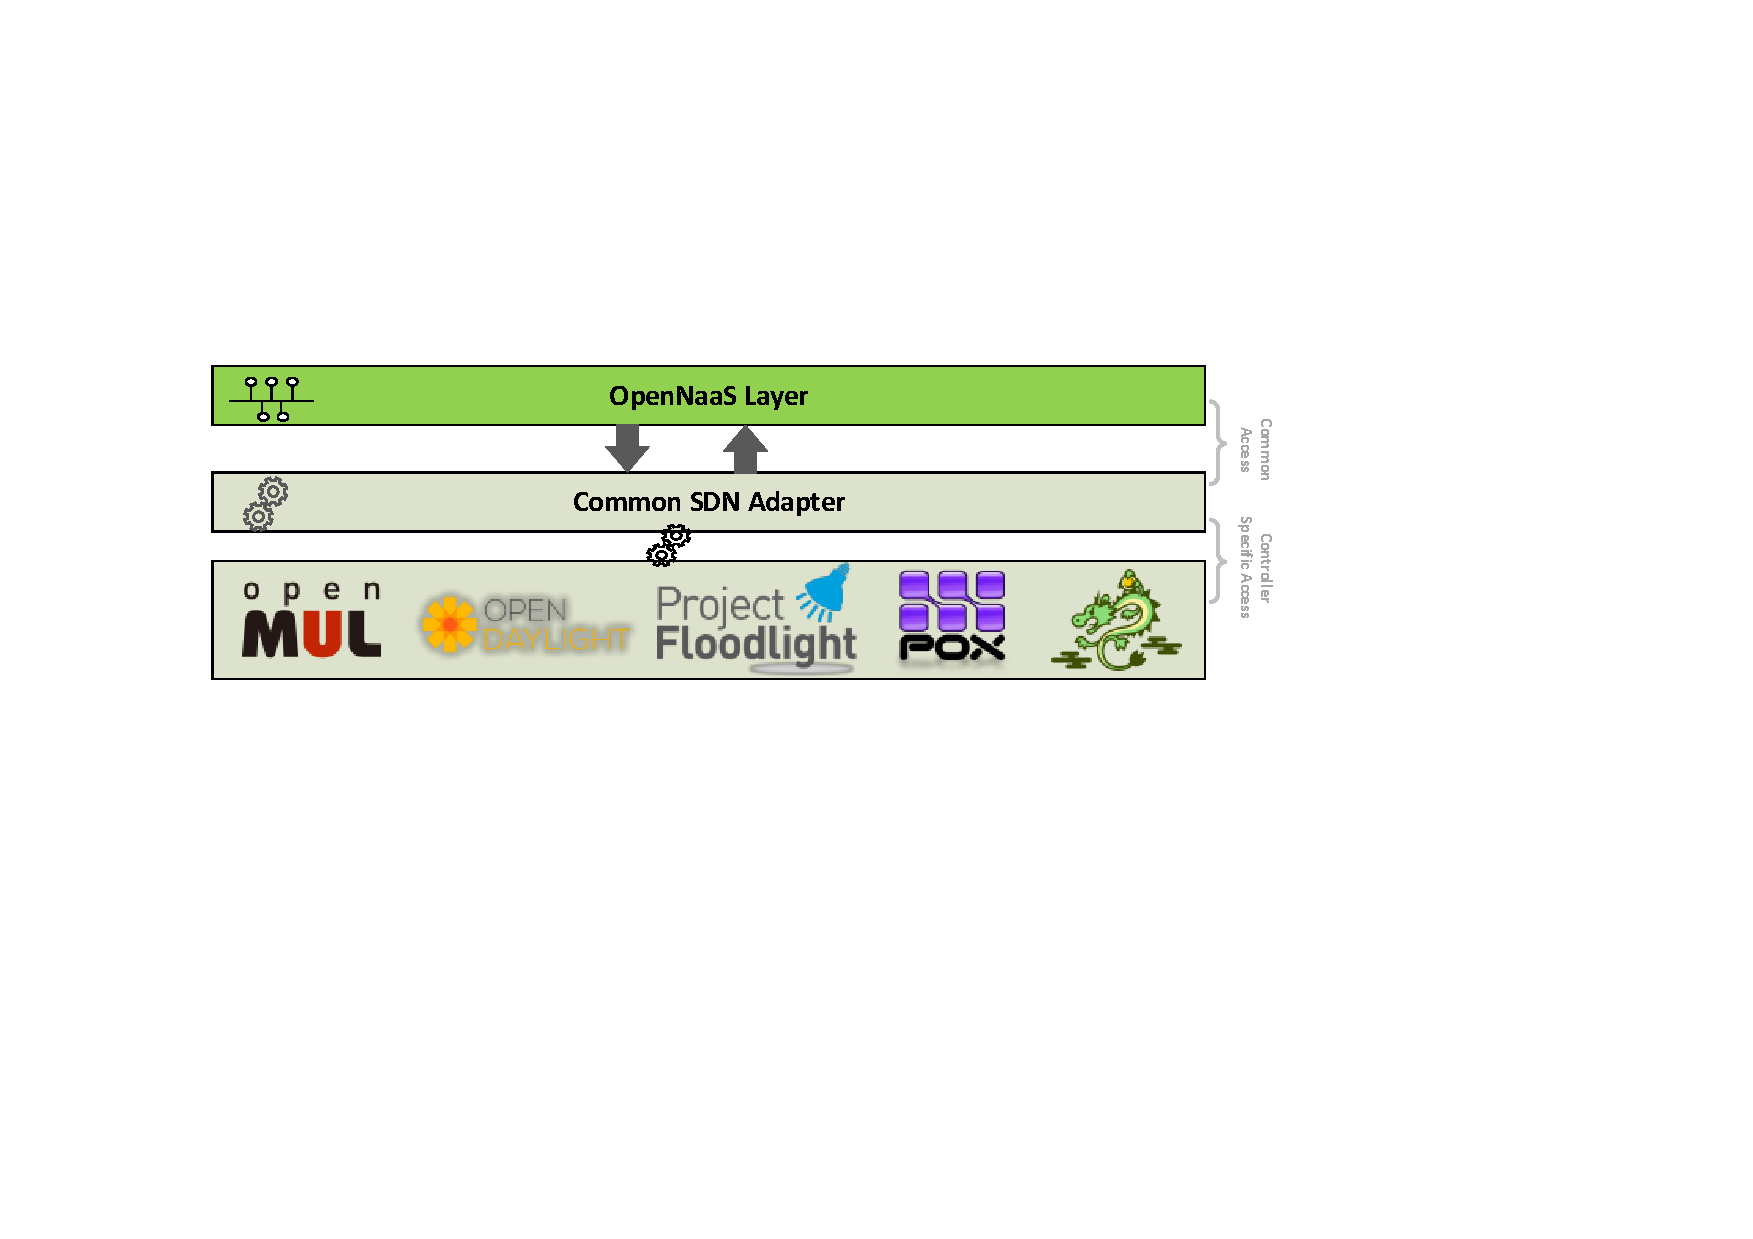
\includegraphics[scale=0.5]{controller-layer.pdf}
	\label{fig:controller-layer}
	\caption{Interactions between NaaS layer and SDN controller layer through a generic adapter}
\end{figure}


In this section, we provide detailed analysis and present our proposals for
service primitives and communication protocols between and across layers.

\subsubsection{Resource Layer Primitives \& Protocols} Service primitives of
this layer towards upper layer are defined by the OF specification from the
Open Networking Foundation (ONF). The main task for the SDN a device is
forwarding data packets in terms of flow according to flow tables and registers
network events such as incoming of data packets that do not match any
pre-defined flow rules. Contrast to conventional ones, flow tables of
SDN-capable devices can be modified at any time point by a controller. In terms
of SDN, a southbound interfaces implements OF specifications and dictates
device-to-controller communications. Note that according to specific
technologies used for the resource layer, reconfigurable protocols other than
OF can be applied as resource layer primitives~\cite{first2013}.

\subsubsection{Control Layer Primitives \& Protocols} A SDN controller exposes
its service primitives through its northbound interfaces. Unlike southbound
interfaces, definition of northbound interfaces is not standardized, it's
depends solely on the different concrete controller implementations what
services primitives in terms of API are considered. In order to make our
solution generic for all controllers, we identify a set of interfaces with
functionalities that are critical for the network management that cover
complete life-cycle of services. Provided with such information, we design an
overarching framework by applying software design
patterns~\cite{gamma1994design}. Some of potential candidates are for example
adapter, proxy and abstract factory patterns. Fig.~\ref{fig:controller-layer} illustrates 
interactions between NaaS layer and diverse controllers through a common SDN adapter.

A further issue concerning control layer protocols is the inter-domain
capability of controllers. Current specification unfortunately does not support
establishing SDN segments across multiple domains thus does not
scale~\cite{scalability2013}. Even within a domain, orchestration of multiple
controller instances are not yet well-defined. This is due the inherent
characteristics that OF based SDN is proposed and created for campus
networks~\cite{openflow08}. In order to sustain this inter-domain capability,
the current protocols have to be extended in Fig.~\ref{fig:arch} we illustrated
this extension as East-West (EW) protocol. To tackle this problem, we envision
two potential approaches:

\begin{itemize}
	\item \textit{Flow Exchanges Protocols.} To improve scalability and
		robustness of SDN based infrastructures, multiple controllers which are
		capable of exchanging informations with each others can be used to
		allow inter-controller communications and maintain a global state of
		the composed networks. To serve this goal, a EW protocol must be in
		place. Due to the differences between inter- and intra-domain
		connections, we distinguishing two types of EW protocols, respectively.

	\item \textit{Global SDN Exchange} In order to allow peering of domains in
		the global level, we propose a SDN exchange instance that allows
		exchanges of flow lables between registered SDN domains.  

\end{itemize}

\subsubsection{NaaS Service Layer Primitives \& Protocols}


\subsubsection{Virtual Connection Layer Primitives \& Protocols}


\section{Implementation/Verification}
	\label{impl}


\section{Further Challenges and Future Work}
	\label{future}


\section{Conclusion}


\section*{Acknowledgment}

\bibliographystyle{IEEEtran}
\bibliography{sdnmo14}

\end{document}
